\documentclass[10pt, a4paper]{jsarticle}

\usepackage{url}
\title{モンテカルロ木探索における\\シミュレーションのGPUを用いた並列化}
\author{明治大学理工学部情報科学科\\知的情報処理システム研究室\\4年15組28番 高野昂平}
\date{}

\usepackage[dvipdfmx]{graphicx}

\begin{document}
\maketitle
\newpage
\tableofcontents
\newpage
\section{はじめに}
\subsection{研究概要}
モンテカルロ木探索(Monte Carlo Tree Search, MCTS)におけるシミュレーション部分を並列化し、高速化を目指す。
% MCTSがなぜ重要なのか、処理速度を上げる事の何がうれしいのか。
\par モンテカルロ木探索は、ゲームにおいて次の強い一手の決定に用いられるだけでなく、ロボットの経路探索や分子構造の設計など幅広く活用される探索アルゴリズムである。処理速度を向上させることによって、同じ処理時間でも処理速度を上げたモンテカルロ木探索はより深く探索を行うことが可能となり、これによって、精度の高い探索を行うことができる。
\par 本研究においては、ゲームのオセロ(リバーシ)を対象に実験を行い、並列化によってどれくらいの速度向上を得られたのか、また、並列化によってプレイヤーの強さがどれくらい向上したのかを検証した。
\subsection{研究背景}
モンテカルロ木探索の処理速度向上を図るうえで、シミュレーション部分が全体の処理速度のボトルネックとなっているのではと考え、シミュレーション部分を並列化することが全体の高速化につながるのではないかと考えた。\par
高性能なCPUを用いることで高速化を図ることも考えられるが、近年CPUの性能向上率が以前に比べて伸び悩んでいるため、CPUを用いない別の手法を試す必要がある。また、一方でGPUの演算性能は演算内容によってはCPUを上回るものとなっている。演算性能の指標としてFLOPS(Floating-point Operations Per Second)があり、1秒間に浮動小数点演算が何回可能であるかを示すが、この値がCPUでは数百GFLOPS程度であるのに対してGPUではそのコア数の多さからPFLOPSに達するものも多い。
% 高止まりと何なのか?単純計算において、CPUとGPUの速度差を提示する必要がある。
このGPUの演算性能の高さゆえに、近年、GPUを画像処理だけでなく、汎用計算に用いてGPGPU(Generarl Purpose GPU)として活用する動きも見られるため、モンテカルロ木探索に対してもGPGPUとして活用できないものかと考えた。
\section{関連研究}
福島らは、モンテカルロ木探索の並列化として、Root並列化を実装しており、探索木を並列に探索する手法を提案している\cite{bib:paper1}。この研究では、木探索自体を並列に実行しており、シミュレーションについての並列化がなされていない点で異なっている。また、美添らは、ハッシュ表を用いた並列化手法を提案している\cite{bib:paper2}。この研究も同様に木探索自体を並列に行っている。
\section{モンテカルロ木探索(MCTS)}
\subsection{モンテカルロ木探索とは}
本研究のテーマであるモンテカルロ木探索(Monte Carlo Tree Search, MCTS)とは、乱数を用いた計算手法であるモンテカルロ法を木探索に応用した手法である。
\par まず、評価関数を用いないという特徴を持つため、様々なゲームのプレイヤーに対してモンテカルロ木探索を実装することができる。例えば、General Game Playing(GGP)という汎用ゲームに対して人間の介入なしで強いプレイヤーを作るという試みがあるが、そのプレイヤーとしてモンテカルロ木探索を用いることが可能である。
\par また、不要な探索を行わないという特徴を持つ。合法手が膨大なゲームに対して木探索を行う場合、そのすべてのノードを探索することによって強いプレイヤーの作成するのは計算量が多くなってしまい、現実的でない。例えば、本研究ではオセロのプレイヤーに対して、モンテカルロ木探索を施したが、そのオセロの合法手は$10^{28}$手あると推測されており、すべてのノードを探索することが困難であることがわかる。しかし、モンテカルロ木探索の場合、すべてのノードを探索するのではなく、有効と考えられる手を優先的に深く探索するため、無駄な探索をすることがなく、計算量を削減することができる。
\par モンテカルロ木探索の流れとしては、選択、シミュレーション、展開、逆伝播の4ステップからなっており(図\ref{fig:parallel})、本研究では2ステップ目のシミュレーションを並列化することを目標としている。
\subsection{UCTについて}
選択ステップにおいて、次に訪問するノードを決めるアルゴリズムとして、UCTアルゴリズムを採用した。このアルゴリズムは、以下の式が最大となるようなノードを次の訪問ノードとするアルゴリズムである。
\par 以下の式において、$w$はそのノードにおける評価値、$n$はそのノードにおける訪問回数、$N$はそのノードを親としたと きの子ノードの$n$の値の合計値、$C$は任意の値で探索がうまくいくように調整すべきパラメータとなっている。
\begin{eqnarray}
    UCT = \frac{w}{n} + C\sqrt{\frac{\ln{N}}{n}}
\end{eqnarray}
\par
この式が意味するのは、ノードの評価値だけで訪問先を決めるのではないということで、第1項自体は評価値の平均を取っているが、第2項において訪問回数が少ないノードを訪問するようにUCT値を調整しているのがわかる。変数$C$はこの訪問回数の少ないノードへの訪問をどれくらい重く見るべきか定めるパラメータと言える。
\section{並列化}
\subsection{並列化による影響}
% 利点と欠点を明確にする。並列化によって起きることの予想を書く。
シミュレーション部分の並列化によって、逐次での実行においてシミュレーションの内容によってはプレイアウト数を増やすことが、実行時間の大幅な増加を招いてしまい、困難であった。しかし、並列化によって実行時間の大幅な削減が可能となるため、プレイアウト数を増やすことができ、より精度の高い探索を行うことが可能となる。
\par しかし、少ないプレイアウト数で実行する場合、1コアあたりの処理性能ではCPUの方が高いため、並列化することでかえって処理速度を遅くしてしまう。
\subsection{手法}
本研究では、シミュレーション部分を並列化するが、具体的には以下の図\ref{fig:parallel}のように、4ステップあるモンテカルロ木探索の2ステップ目を複数回のシミュレーションを同時に実行することで実現する。
\begin{figure}[ht]
    \begin{center}
        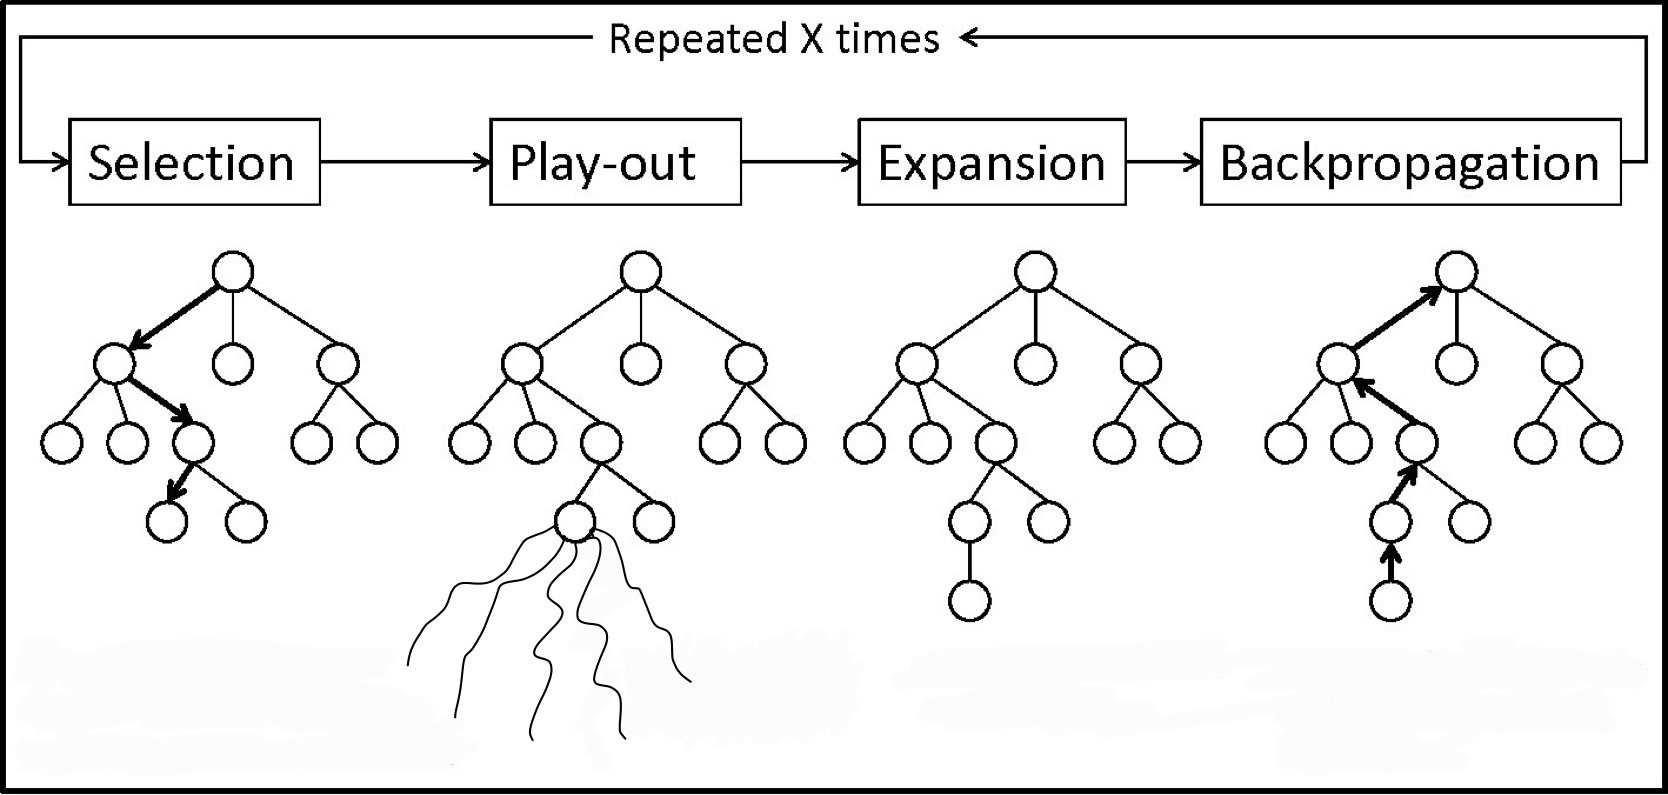
\includegraphics[width=15cm]{img/mcts_parallel.jpg}
        \caption{シミュレーションの並列化\cite{img:parallel}} \label{fig:parallel}
    \end{center}
\end{figure}
\par 複数回のシミュレーションを行う際、CPUでの逐次実行とGPUでの並列実行の違いは、まず、逐次実行の場合には図\ref{fig:cpu_mcts_code}のように1回のシミュレーションをfor文によって複数回順番に実行し、それぞれのシミュレーションで得た値を足し合わせることで処理を行っている。
\par 一方、並列実行の場合、図\ref{fig:gpu_mcts_code}のように1回のプレイアウト関数の呼び出しによって、複数回のシミュレーションを終えている。厳密には、playout\_cuda関数内でのカーネル呼び出しによって並列にシミュレーションが行われる。
\begin{figure}[ht]
    \begin{center}
        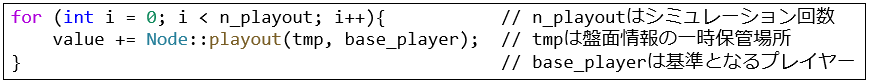
\includegraphics[width=15cm]{img/cpu_mcts_code.png}
        \caption{CPUによる逐次実行}
        \label{fig:cpu_mcts_code}
    \end{center}
\end{figure}
\begin{figure}[ht]
    \begin{center}
        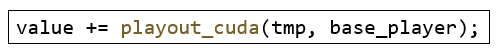
\includegraphics[width=12cm]{img/gpu_mcts_code.png}
        \caption{GPUによる並列実行}
        \label{fig:gpu_mcts_code}
    \end{center}
\end{figure}
\section{実験環境}
\subsection{パラメータについて}
ある盤面ノードに対する評価回数(図\ref{fig:parallel}におけるX)を100回、ノードの展開の基準値を20回訪問とした。また、CUDAカーネルを1ブロックあたりのスレッド数を512として、実験を行った。
\subsection{並列化環境について}
並列化にあたって、NVIDIA社のCUDA(Compute Unified Device Architecture)を用いた。CUDAはNVIDIA社のGPU上で動作する汎用並列コンピューティングプラットフォームである。なお、言語はC++とし、CUDA Cを用いて実装を行った。
\subsection{実行環境}
CUDAを用いる関係上、GPUはNVIDIA社のものとなっている。
\begin{table}[ht]
    \begin{center}
        \begin{tabular}{ll}
            OS & Ubuntu 20.04.2 LTS \\
            CPU & Intel(R) Core(TM) i9-10900X CPU @ 3.70GHz \\
            GPU & GeForce RTX 3080 (CUDAコア 8704)\\
            メモリ & 32GB \\
        \end{tabular}
    \end{center}
\end{table}
\section{実行速度の計測}
\subsection{実験概要}
実験の流れとしては、オセロの初期盤面における評価(図\ref{fig:parallel}における1サイクル)を100回行う。それぞれの評価を行う中で、CPUでのシミュレーションとGPUでのシミュレーションを実行する。各シミュレーションで実行時間を計測し、100回分の実行時間を計測し終わった後、それらの平均を求める。この平均をもとに実行時間の比較を行った。
\par この実験によって、CPUでのシミュレーションに対してGPUでのシミュレーションがどの程度高速化できているのかを見ていく。また、GPUで並列化をしたとしても、同時に並列実行できる数には限りがあり、プレイアウト数を増やし続けるとGPUでのシミュレーションにおいても実行時間が増えていくことが予想される。よって、GPUでのシミュレーションにおいてプレイアウト数を増やしていくことで、どれくらい実行時間が増加していくのかについても見ていく。
\subsection{実行時間の比較}
\begin{figure}[ht]
    \begin{center}
        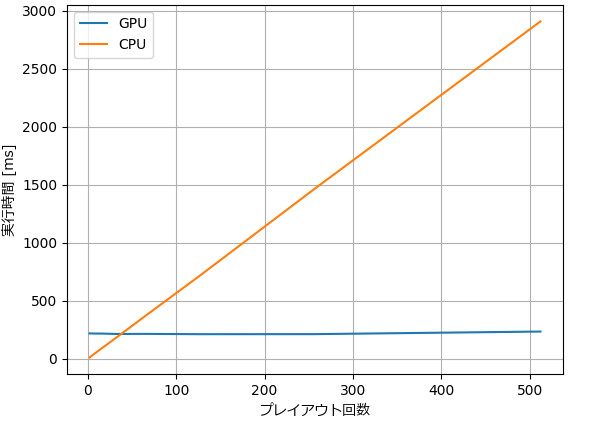
\includegraphics[width=12cm]{img/gpu_cpu_time.png}
        \caption{実行時間の比較}
        \label{fig:cpu_gpu_time}
    \end{center}
\end{figure}
\par 図\ref{fig:cpu_gpu_time}はプレイアウト数を1から順に2倍ずつ増やしたときの、実行時間の変化をグラフにしたものである。
\par 図\ref{fig:cpu_gpu_time}からわかるように、CPUの逐次実行での実行時間が線形的に増加しているのに対して、GPUでの実行時間は並列処理であるため、実行時間が増えていない。また、プレイアウト数が少ないときには、並列実行よりもCPUでの逐次実行の方が実行時間が短く、並列化による高速化はある程度のプレイアウト数が必要になることがわかる。
\subsection{並列処理の実行時間の増加について}
\begin{figure}[ht]
    \begin{center}
        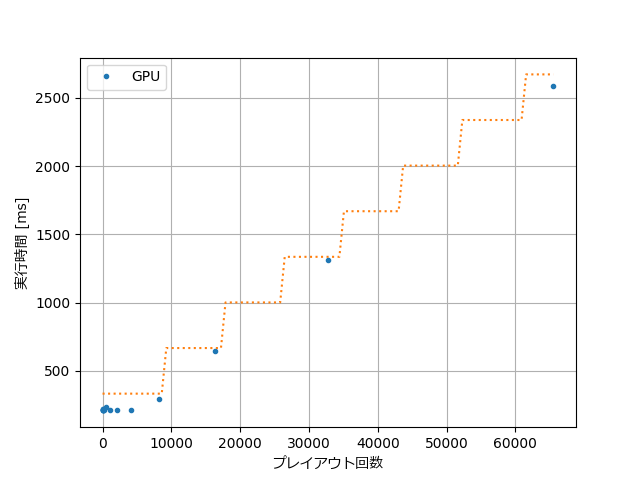
\includegraphics[width=12cm]{img/gpu_time_wCeil.png}
        \caption{GPUでの実行時間}
        \label{fig:gpu_time}
    \end{center}
\end{figure}
\par 図\ref{fig:gpu_time}は、さらにプレイアウト数を増やした場合のGPUでの実行時間の変化をグラフにしたものである。本実験ではプレイアウト数を2倍ずつ増やしているため、その実行時間をグラフにした際に、線形的に増加しているように見える。しかし、プレイアウト数を細かく変化させ、実行時間を計測した場合、天井関数に近い形のグラフになることが予想される。本実験で用いたGPUのCUDAコア数が8704であるため、プレイアウト数が8704大きくなるごとに実行時間が増加していくことが予想され、プレイアウト数が8704大きくなるごとに次の値を取るような天井関数は$f(x) = a\left\lceil\frac{x}{8704}\right\rceil$となる。この時、$a$は実行時間の増加幅にあたる。この値は、実際に計測して得た実行時間をもとに適切な値を設定した。具体的には、隣り合った計測点2点の実行時間の差分$\Delta t$とプレイアウト数の差分$\Delta p$を取り、すべての$\frac{\Delta t}{\Delta p}$の平均を8704倍することで$a$を算出した。ただし、プレイアウト数の差分が8704未満のものは実行時間の差がないことが予想され、平均に含めてしまうと$a$が極端に小さくなってしまうため、この平均に含めない。そして、これらの値をもとに予想される天井関数の概形が図\ref{fig:gpu_time}における点線部分にあたる。
% どのようにして予測線を引いたのかを明確にする。
\par 並列に実行した場合でも、プレイアウト数を増やしていくとCPUでの逐次実行と同様に実行時間が増えていくことがグラフから見て取れるが、しかし、その増加幅はCPUでの逐次実行に比べて緩やかなものとなっており、このままプレイアウト数を増やしたとしても、並列処理での実行時間の短縮は実現できるものと考える。
\section{強さの比較}
\subsection{実験概要}
プレイアウト数を増やすことでプレイヤーがどれくらい強くなるのか実験を行った。
\par 逐次実行ではプレイアウト数を増やして実行すると実行時間が大きく増加し、プレイアウト数の増加に伴うプレイヤーの強さの変化を見るのが難しかったが、並列化を施したことでプレイアウト数を増やしたときにどれくらいプレイヤーが強くなるのか見ることができる。また、プレイアウト数を増やすことでより正確な評価値を得ることができるが、ある程度のプレイアウト数があれば、それ以上増やしても大きく強さに影響しないのではないかと考えた。よって、本実験においては強さの変化と強さの上限について調べる。
\par 後手白の強さを固定し、先手黒のプレイアウト数を増やしていったときにどのように勝率が変化するかを見ていくことで強さの評価を行った。後手白の強さはプレイアウト回数を2048回とした。
\subsection{検定について}
本実験を行う上でt検定を行い、勝率を評価した。帰無仮説を"先手黒と後手白の強さは同じ"とし、また、対立仮説を"白が黒より強い"とした。対立仮説をこのようにしたのは、今回の実験において後手白のプレイアウト回数が先手黒のプレイアウト回数より多いことが保証されており、白の強さが黒を下回ることは予想されないためである。この対立仮説を示すために片側検定を行った。よって、有意水準を0.05としたとき、z値が-1.64を下回る勝率に関しては帰無仮説を棄却し、対立仮説を採用するため"白が黒より強い"ということが有意に言える。
\subsection{勝率の評価}
\begin{table}[ht]
    \begin{center}
        \begin{tabular}{c|c|c|c|c}
            プレイアウト数 & 勝ち数 & 負け数 & 勝率[\%] & z値 \\ \hline
            1 & 4 & 146 & 2.67 & -11.59 \\
            2 & 18 & 131 & 12.08 & -9.26 \\
            4 & 27 & 120 & 18.37 & -7.67 \\
            8 & 36 & 113 & 24.16 & -6.31 \\
            16 & 55 & 94 & 36.91 & -3.2 \\
            32 & 65 & 84 & 43.62 & -1.56 \\
            64 & 64 & 82 & 43.84 & -1.49 \\
            128 & 81 & 69 & 54.00 & 0.98 \\
            256 & 74 & 72 & 50.68 & 0.17 \\
            512 & 67 & 81 & 45.27 & -1.15
        \end{tabular}
        \caption{勝率}
        \label{tab:win_rate}
    \end{center}
\end{table}
\par 表\ref{tab:win_rate}より、プレイアウト回数を1回のとき、先手黒が後手白より圧倒的に弱いことがわかる。徐々にプレイアウト回数を増やしていくと後手白の強さに近づいていく。特に、プレイアウト回数128回及び256回では、先手黒のプレイアウト回数が後手白よりも少ないにも関わらず勝ち越しているため、ある程度のプレイアウト回数があれば、それ以上増やしても強さに大きな影響はないといえる。つまり、32回ほどのプレイアウト数があれば、強さの上限を迎えることが本実験でわかった。
% プレイアウト回数が同じ場合50%の勝率が予想される。予想と結果の比較を書く。
\section{おわりに}
本研究によって、まず、シミュレーションの並列化によって逐次での複数回シミュレーションに比べて、大幅に実行時間を短縮することができた。実行時間の短縮によって、単位時間当たりのプレイアウト数が増加するため、より精度の高い木探索を行うことにつながる。
\par また、プレイアウト数の増加に伴う強さの変化を検証した。この実験では、強さの変化を見るとともに強さの上限を検証した。強さの変化自体は、プレイアウト数1から始まり、徐々に強くなることがわかった。しかし、プレイアウト数が32回あたりに達すると2048回プレイアウトのプレイヤに対して、同じくらいの強さになったため、プレイアウト数が32回ほどで強さの上限を迎えることがわかった。
% ゲーム木が複数できるとは何なのかわかるように説明する。
\par モンテカルロ木探索におけるシミュレーション部分を並列化することができたため、逐次実行ではプレイアウト数を増やしたとき、実行時間が膨大となっていたところを大幅に短縮することができた。しかし、プレイアウト数を増やしたとしても、ある程度のプレイアウト数で強さに限界を迎えてしまう。よって、今後の課題としては、モンテカルロ木探索の別箇所の並列化を行い、より強くより速いプレイヤーを作る必要がある。モンテカルロ木探索において他に並列化できそうな箇所としては評価を並列に行うことが考えられる。つまり、ある盤面ノードに対して100回の評価を並列に実行し、例えば、並列数が10個の場合、1000回の評価に相当するゲーム木を生成できるのではないかと考えた。しかし、評価関数の複数回実行を並列化するためには、100回の評価によって得られたそれぞれのゲーム木を1つのゲーム木に統一する必要があるため、この統一する手法について考える必要がある。
\begin{thebibliography}{99}
    \bibitem{img:parallel} Monte Carlo Tree Search in Lines of Action(一部改変), \url{https://www.semanticscholar.org/paper/Monte-Carlo-Tree-Search-in-Lines-of-Action-Winands-Bj%C3%B6rnsson/5575020996d239acbdd9c17f6239a4bca027aa88}
    \bibitem{bib:paper1} 福島祐介, 岸本 章宏, 渡辺 治, "モンテカルロ木探索のRoot並列化とコンピュータ囲碁での有効性について", ゲームプログラミングワークショップ2009論文集, 2009-11-06
    \bibitem{bib:paper2} 美添一樹, 石川 裕, "分散並列モンテカルロ木探索フレームワークの提案", 研究報告ハイパフォーマンスコンピューティング(HPC), 2010-07-27
\end{thebibliography}
\end{document}